\documentclass[12pt,letterpaper, onecolumn]{exam}
\usepackage{amsmath}
\usepackage{amssymb}
\usepackage{graphicx}
\usepackage[lmargin=71pt, tmargin=1.2in]{geometry}
\lhead{EN.625.252.81 Fall 2025\\}
\rhead{Haadi Majeed\\}
% \chead{\hline}
\thispagestyle{empty}

\begin{document}

\begingroup  
    \centering
    \LARGE EN.625.252.81 Fall 2025\\
    \LARGE Module 2 Assignment\\[0.5em]
    \large \today\\[0.5em]
    \large Haadi Majeed\par
    \large hmajeed01\par
    \large Due Sunday September 7th at 10:59 CST\par
\endgroup
\rule{\textwidth}{0.4pt}
% \pointsdroppedatright
\printanswers
\renewcommand{\solutiontitle}{\noindent\textbf{Ans:}\enspace}

\begin{center}
    In the problems below let
    $A = \begin{bmatrix}
    1 & 1 & 0 \\
    1 & 2 & 1 \\
    0 & 1 & 1
    \end{bmatrix}$
\end{center}
\begin{questions}
    
    \question Calculate $rref(A)$ by hand showing all the steps of your row reduction.
    \begin{solution}
        \begin{center}
            $\begin{bmatrix}
                1 & 1 & 0 \\
                1 & 2 & 1 \\
                0 & 1 & 1
            \end{bmatrix}$
            \\$\downarrow$\\
            $R_2 \leftarrow R_2 - R_1$\\
            $\begin{bmatrix}
                1 & 1 & 0 \\
                1 - 1 & 2 - 1 & 1 - 0 \\
                0 & 1 & 1
            \end{bmatrix}$
            \\$\downarrow$\\
            $\begin{bmatrix}
                1 & 1 & 0 \\
                0 & 1 & 1 \\
                0 & 1 & 1
            \end{bmatrix}$
            \\$\downarrow$\\
            $R_1 \leftarrow R_1 - R_2$\\
            $\begin{bmatrix}
                1 - 0 & 1 - 1 & 0 - 1 \\
                0 & 1 & 1 \\
                0 & 1 & 1
            \end{bmatrix}$
            \\$\downarrow$\\
            $\begin{bmatrix}
                1 & 0 & -1 \\
                0 & 1 & 1 \\
                0 & 1 & 1
            \end{bmatrix}$
            \\$\downarrow$\\
            $R_3 \leftarrow R_3 - R_2$\\
            $\begin{bmatrix}
                1 & 0 & -1 \\
                0 & 1 & 1 \\
                0 - 0 & 1 - 1 & 1 - 1
            \end{bmatrix}$
            \\$\downarrow$\\
            $rref(A) =
            \begin{bmatrix}
                1 & 0 & -1 \\
                0 & 1 & 1 \\
                0 & 0 & 0
            \end{bmatrix}$
        \end{center}
        
    \end{solution}
    \pagebreak

    \question Using your answer to 1, determine the general solution of $Ax = 0$.    
    \begin{solution}
        \begin{center}
            $Ax=0$\\
            $\begin{bmatrix}
                1 & 0 & -1 \\
                0 & 1 & 1 \\
                0 & 0 & 0
            \end{bmatrix}
            *
            \begin{bmatrix}
                x_1\\
                x_2\\
                x_3
            \end{bmatrix}
            =
            \begin{bmatrix}
                0\\
                0\\
                0
            \end{bmatrix}$\\
            $x_1 - x_3 = 0$\\
            $x_2 + x_3 = 0$\\
            $0 = 0$\\
            $\therefore$\\
            $x_1 = x_3$\\
            $x_2 = -x_3$\\
            $x_3$ is a free variable\\
            $x_3 = t$\\

            $x = \begin{bmatrix}
                x_1\\
                x_2\\
                x_3
            \end{bmatrix}
            =
            \begin{bmatrix}
                x_3\\
                -x_3\\
                x_3\\
            \end{bmatrix}\ or\ 
            \begin{bmatrix}
                t\\
                -t\\
                t
            \end{bmatrix}\ or\
            t \begin{bmatrix}
                1\\
                -1\\
                1
            \end{bmatrix}
            $\\
            where $t \in \mathbb{R}$\\
        \end{center}

    \end{solution}
    \pagebreak

    \question Solve the matrix equation
        $Ax = \begin{bmatrix}
            1 \\
            0 \\
            1
        \end{bmatrix}$, or show that no solution exists.
    \begin{solution}
        \begin{center}
            $\begin{bmatrix}
                1 & 1 & 0 & 1\\
                1 & 2 & 1 & 0\\
                0 & 1 & 1 & 1
            \end{bmatrix}
            \begin{matrix}
                \\
                R_2 \leftarrow R_2 - R_1\\
                \ 
            \end{matrix}$\\
            $\begin{bmatrix}
                1 & 1 & 0 & 1\\
                1 - 1 & 2 - 1 & 1 - 0 & 0 - 1\\
                0 & 1 & 1 & 1
            \end{bmatrix}
            =
            \begin{bmatrix}
                1 & 1 & 0 & 1\\
                0 & 1 & 1 & -1\\
                0 & 1 & 1 & 1
            \end{bmatrix}$\\
            $R_1 \leftarrow R_1 - R_2$\\
            $R_3 \leftarrow R_3 - R_2$\\
            $\begin{bmatrix}
                1 - 0 & 1-1 & 0-1 & 1-(-1)\\
                0 & 1 & 1 & -1\\
                0-0 & 1-1 & 1-1 & 1-(-1)
            \end{bmatrix}
            =
            \begin{bmatrix}
                1 & 0 & -1 & 2\\
                0 & 1 & 1 & -1\\
                0 & 0 & 0 & 2
            \end{bmatrix}$\\
            \ \\
            $x_1 - x_3 = 2$\\
            $x_2 + x_3 = -1$\\
            $0 = 2$\\
            This is a contradiction as $0=2$ is invalid and this is inconsistent, No Solution
        \end{center}
    \end{solution}
    \pagebreak

    \question Use 3D graphing software (e.g. Geogebra or Desmos) to give a geometric description of your answers to problems 2 and 3. (Note: even if a systems is inconsistent, you can still graph to show no common intersection occurring.)
    \begin{solution}
    
        \begin{center}
        This first graph is representative of the problem 2, it can be seen as vector going from the origin (limited) to $(1, -1, 1)$ as it scales with any given $t$ value. The redline highlighting the vector and the two planes from the augmented matrix of $Ax = \begin{bmatrix}
            0\\0\\0
        \end{bmatrix}$
        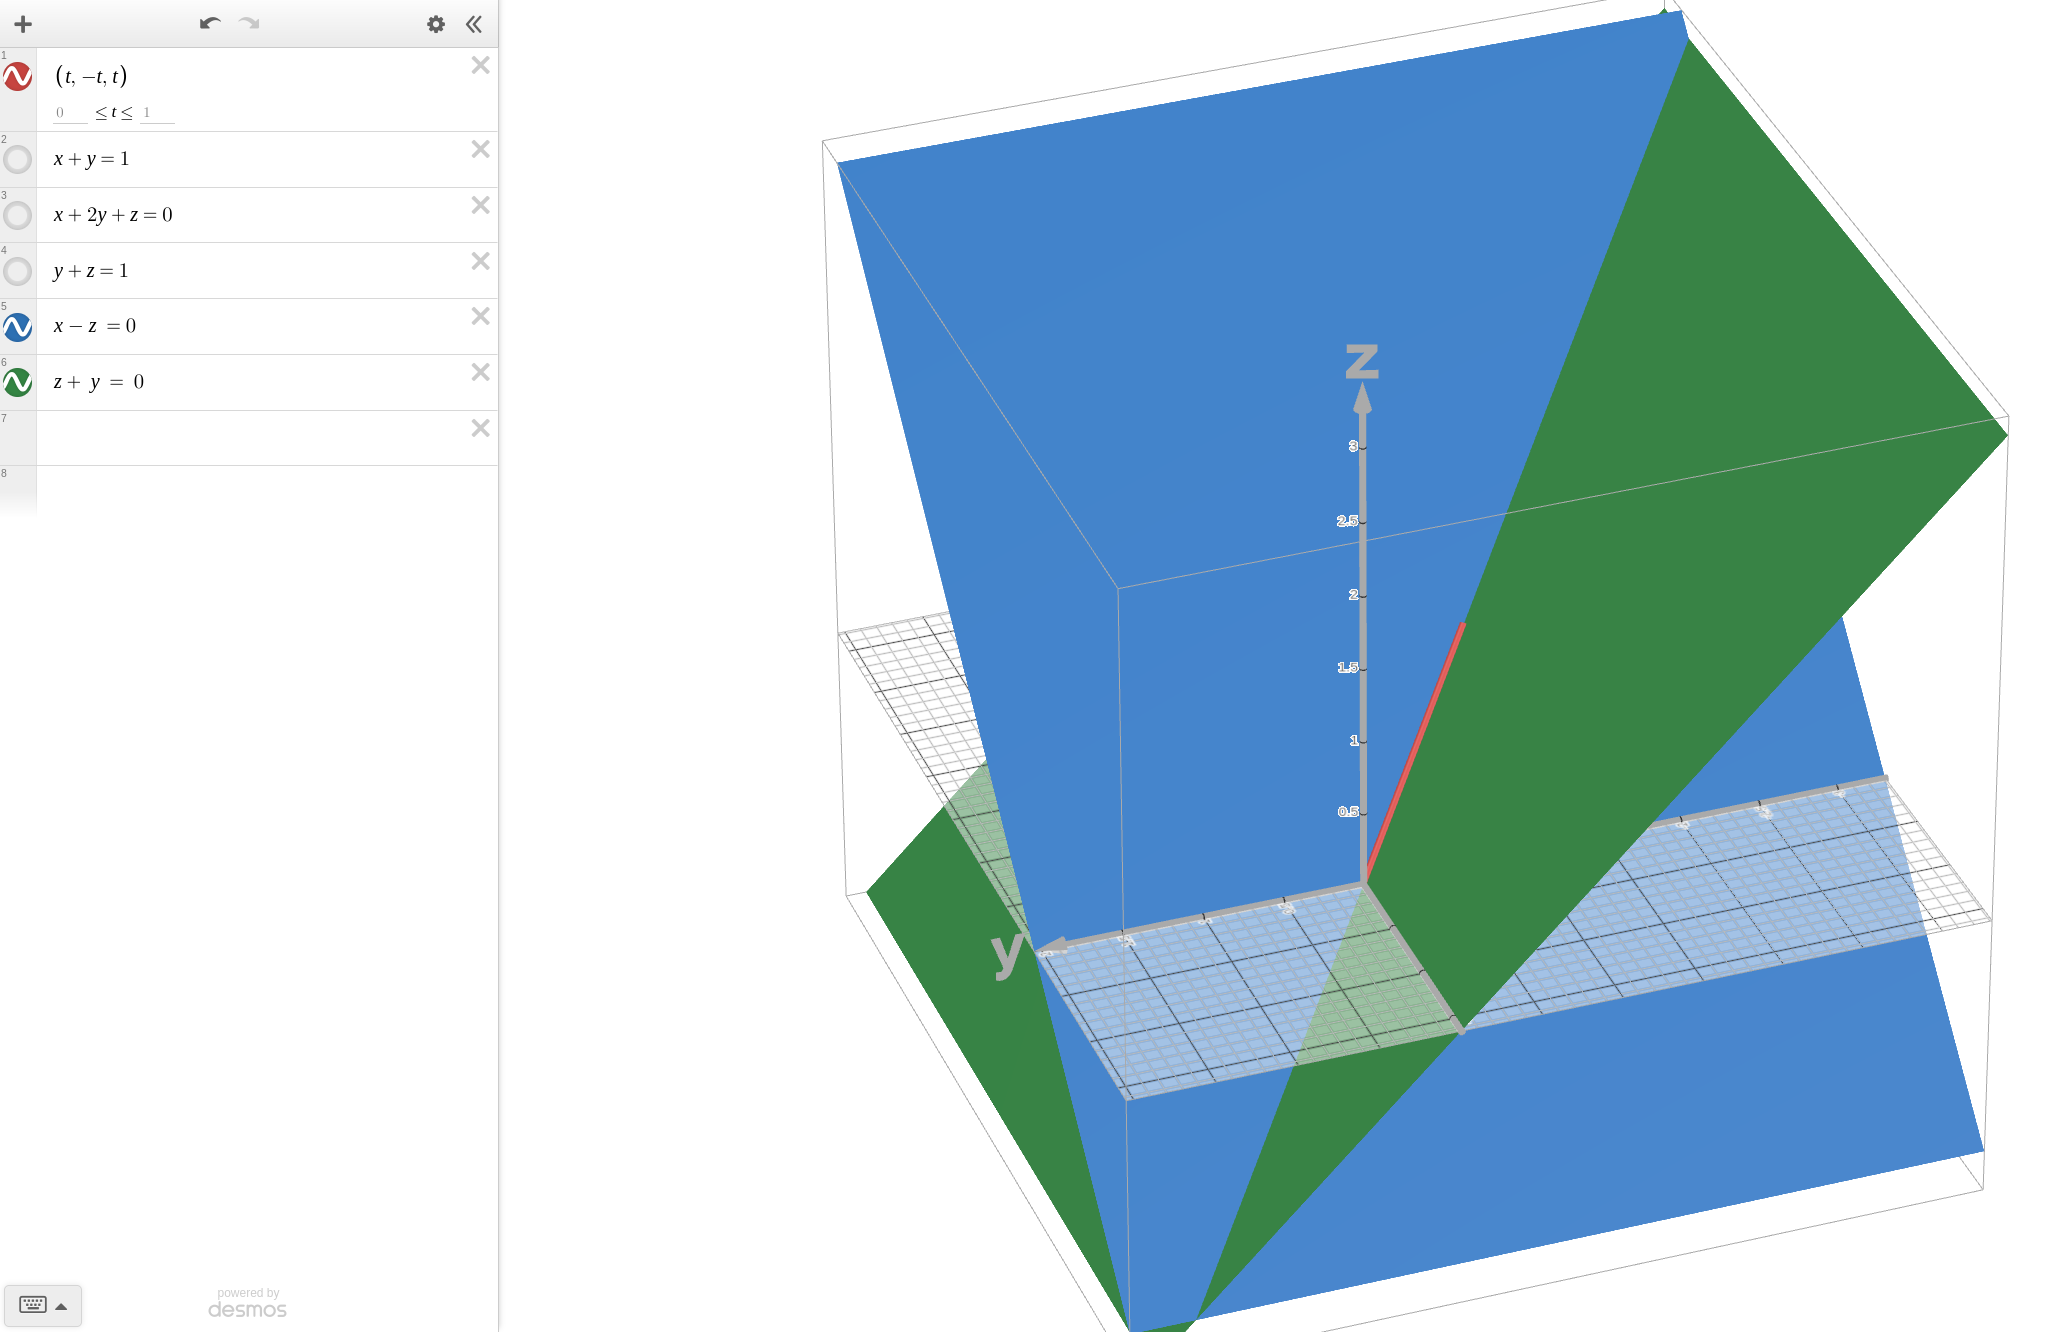
\includegraphics[width=0.8\textwidth]{GraphOfNumber2.png}\\
        This second graph is showing the three equations independently graphed derived from the initial augmented matrix from question 3: $\begin{bmatrix}
                1 & 1 & 0 & 1\\
                1 & 2 & 1 & 0\\
                0 & 1 & 1 & 1
            \end{bmatrix}$ Following the planes outward, there is no point where all three will converge\\
        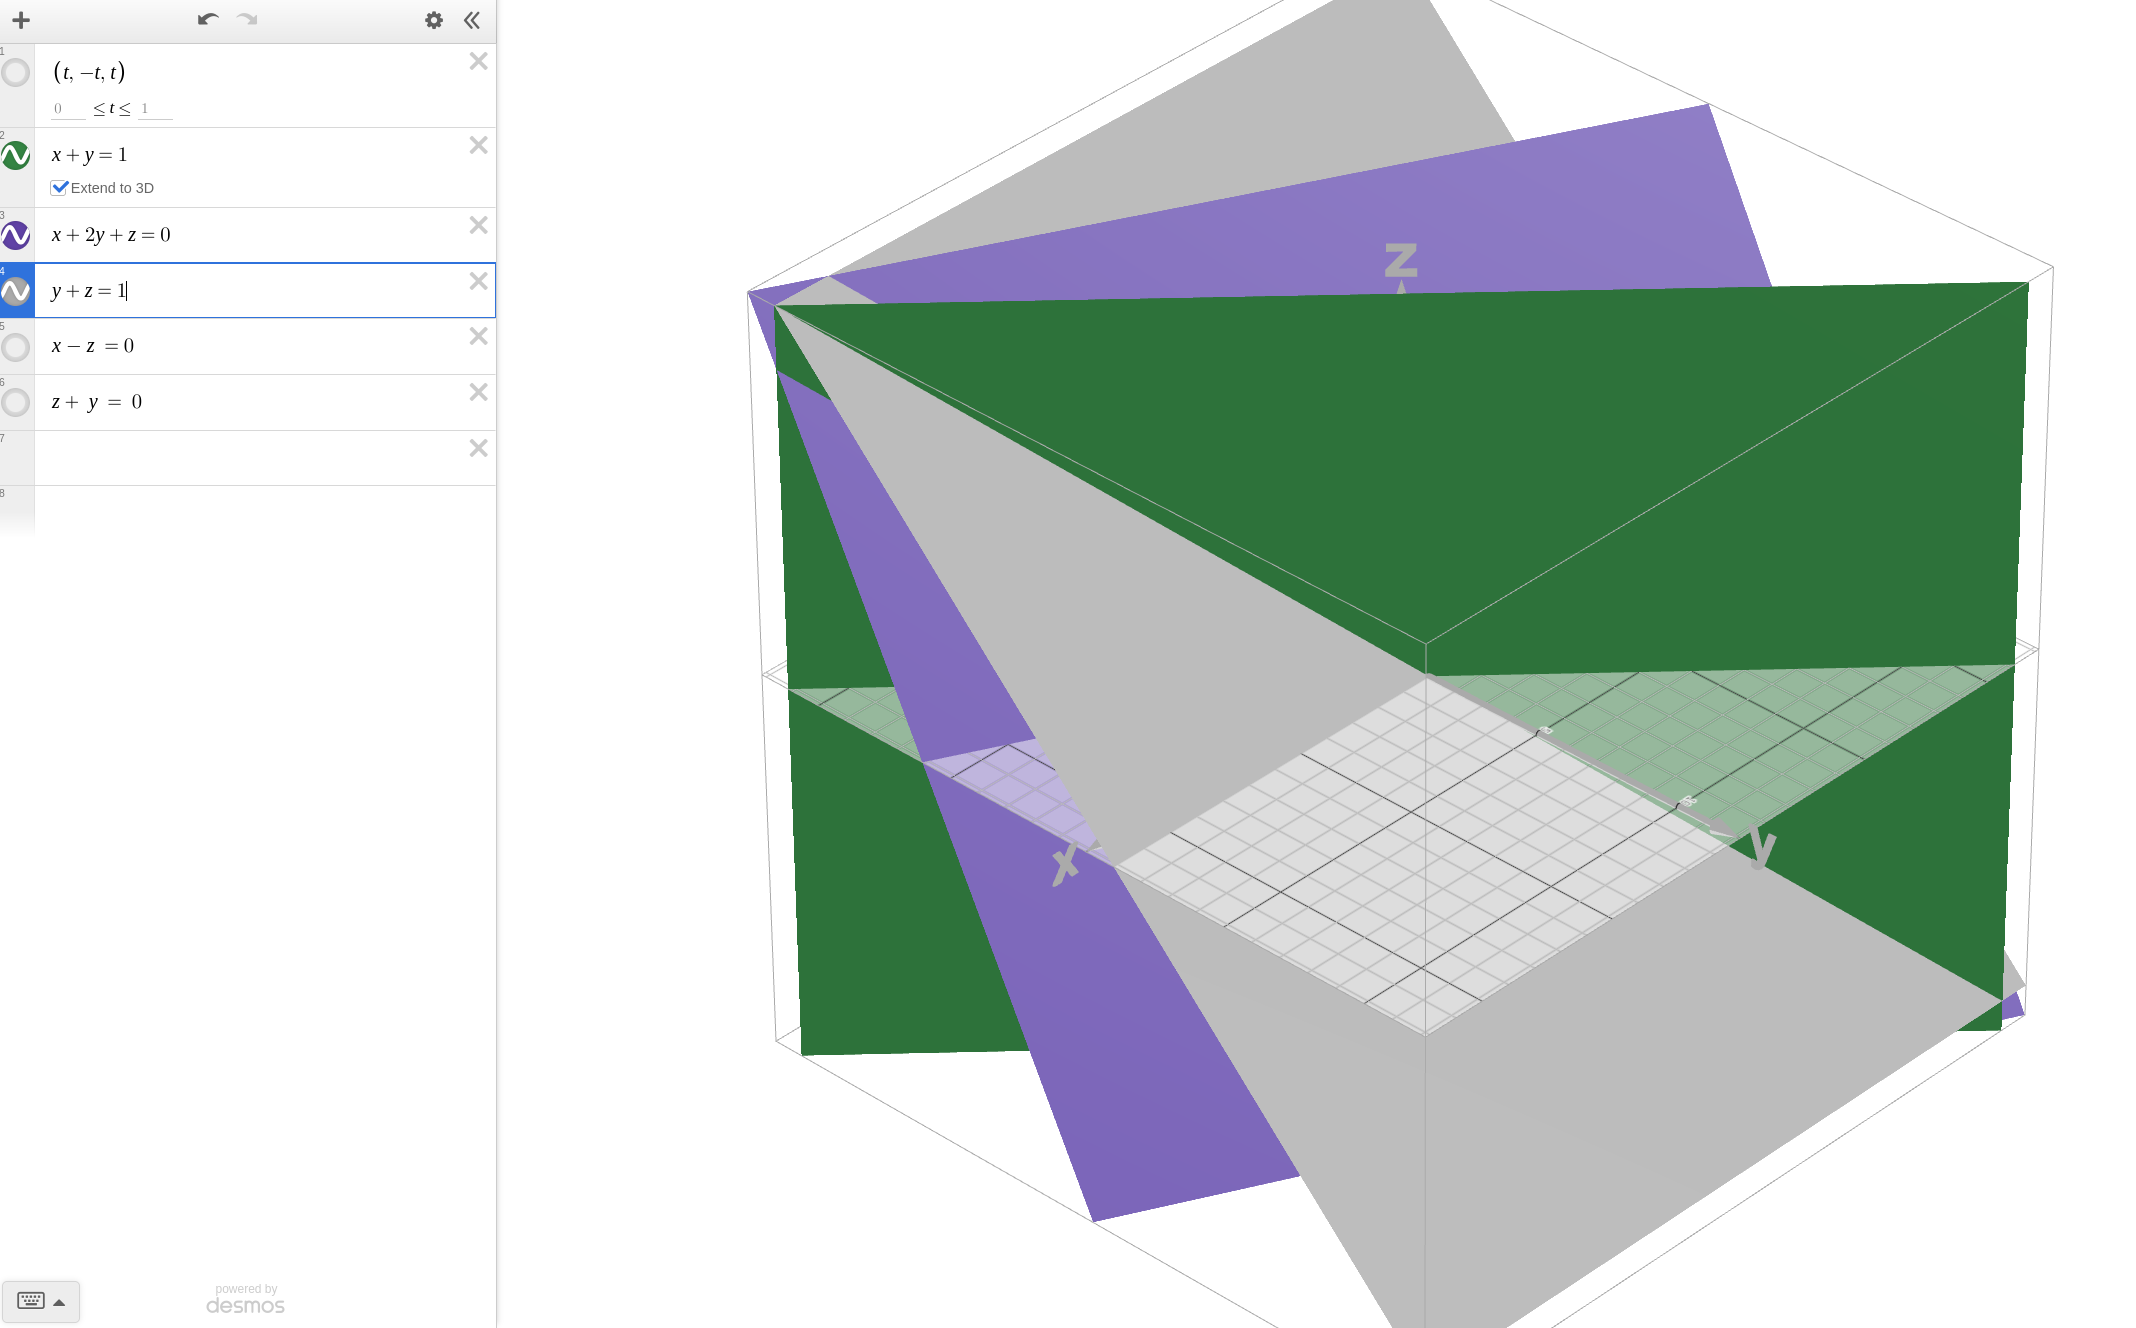
\includegraphics[width=0.8\textwidth]{GraphOfNumber3.png}
    \end{center}
    \end{solution}
    
\end{questions}
\end{document}
